\chapter{Aufgaben}\label{ch:aufgaben}
\section{Allgemeine Aufgabenbeschreibung}\label{sec:aufgaben_allgemein}

Im Rahmen des Praxisprojekts ist die Implementierung eines AI-Chatbots für den
Konfigurator eines Unternehmens für Unterflursysteme geplant.\\ 
Die Aufgaben beginnen mit einer detaillierten Anforderungsanalyse, bei der die Bedürfnisse der
Stakeholder und die spezifischen Use Cases für den Konfigurator definiert werden.\\
Auf dieser Basis erfolgt die Auswahl der geeigneten Technologien und Frameworks
für die Entwicklung des Chatbots.\\\\ Ein zentraler Bestandteil des Projekts ist die
Beschaffung der benötigten Daten aus dem Backend des Unternehmens. Diese
Daten müssen zunächst aufbereitet und in einem passenden Format für die
Verarbeitung strukturiert werden.\\
Anschließend werden die Daten in eine Vektor-Datenbank integriert, um eine
effiziente Suche und Abfrage durch den Chatbot zu ermöglichen.\\Im nächsten
Schritt wird der AI-Chatbot implementiert und trainiert, um Nutzeranfragen im
Zusammenhang mit dem Konfigurator zu beantworten.
Hierbei wird der Chatbot mit der Vektor-Datenbank verbunden, um dynamisch auf
die dort hinterlegten Informationen zugreifen zu können.\\
Zum Abschluss wird eine Dokumentation über das gesamte Projekt erstellt, die die
Implementierung, die Funktionsweise und die Nutzung des Chatbots beschreibt.


\pagebreak
\section{Projektinformationen}\label{sec:proj_info}
\subsection{Unterflursysteme}\label{sec:unterflursysteme}

Unterflursysteme sind eine spezielle Art von Bodentanks, die in Bürogebäuden, Konferenzräumen und anderen öffentlichen Gebäuden eingesetzt werden.  
In diesen Systemen können verschiedene Module wie Steckdosen, Netzwerkanschlüsse, USB-Ports und Multimedia-Anschlüsse integriert werden.\\  
Die Bodentanks werden bündig im Boden verlegt und sind mit einer Abdeckung versehen, die bei Bedarf geöffnet werden kann, um Zugang zu den darin enthaltenen Modulen zu erhalten.\\\\  
Der Kunde, für den der Chatbot entwickelt werden soll, bietet eine Vielzahl von Unterflursystemen an, die individuell konfiguriert werden können.  
Diese Konfiguration umfasst die Auswahl der Art des Tanks (Beton oder Estrich), der Module, die Anzahl der Anschlüsse und die Positionierung der einzelnen Elemente im Bodentank.\\  
Dabei kann die Konfiguration je nach Anforderungen durchaus komplex sein, wobei der Chatbot helfen soll.

\begin{figure}[H]
    \begin{center}
        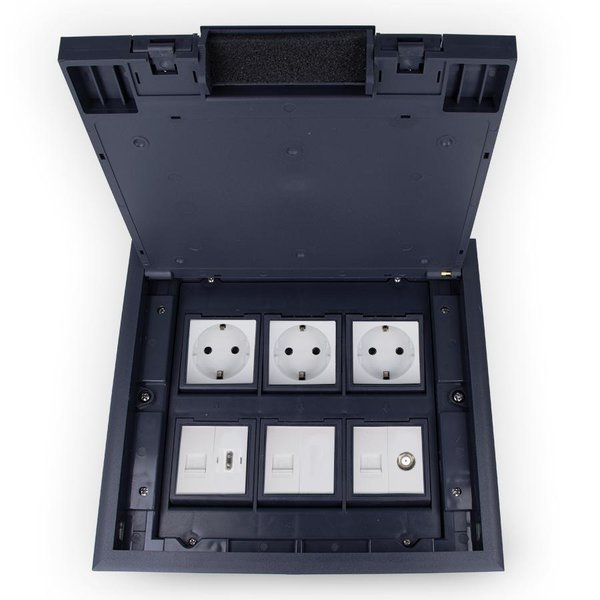
\includegraphics[width=3cm]{bilder/bodentank.jpeg}
        \caption{Beispiel Bild für einen Bodentank}\label{fig:bodentank}
    \end{center}
\end{figure}

\pagebreak
\subsection{Projekttyp}\label{sec:proj_typ}
Der Chatbot soll mit den Methodiken von \gls{rag} entwickelt werden.\\  
\gls{rag} ist ein Ansatz zur Entwicklung von Chatbots, der mit Hilfe der Nutzereingabe  
passende Informationen aus einer Datenbank abruft und mit diesen zusammen eine Antwort generiert.

\subsection{Projektziele}\label{sec:proj_ziele}
Das Ziel des Projektes ist es, einen kosteneffizienten und nützlichen Chatbot zu entwickeln, der Nutzer  
bei der Konfiguration von Unterflursystemen unterstützen kann.\\  
Sollte dies erfolgreich sein und der Kunde überzeugt werden, soll der Chatbot  
möglichst einfach auf weitere Konfiguratoren des Kunden erweiterbar sein.\\\\  
Sehr wichtig war mir dabei, nicht einfach einen weiteren simplen Wrapper für gängige \gls{llm} zu programmieren.  
Diese sind aus meiner Erfahrung und der meiner Arbeitskollegen oft nicht hilfreich und negativ behaftet, insbesondere wenn diese  
anstatt eines kompetenten Support-Teams eingesetzt werden.

Daher waren mir folgende Punkte besonders wichtig:
\begin{itemize}
    \item \textbf{Kosteneffizient.}\\Der Kontext der Produktdaten soll nur die nötigsten Informationen enthalten.
    \item \textbf{Einfache Erweiterbarkeit.}\\Der Chatbot soll möglichst einfach auf weitere Konfiguratoren des Kunden erweiterbar sein.
    \item \textbf{Nutzerfreundlichkeit.}\\Das Design und die Interaktionen sollen möglichst intuitiv sein. Zusammenarbeit mit dem UX-Team.
    \item \textbf{Kein Ersatz für den Support.}\\Der Chatbot soll den Support nicht ersetzen, sondern ergänzen.
\end{itemize}